\documentclass[24pt,a4paper]{article}
\usepackage{graphicx}
\usepackage[english]{babel}
\usepackage{blindtext}
\usepackage{fancyhdr}
\usepackage{blindtext}
\usepackage[table]{xcolor}
\usepackage[a4paper]{geometry}
\usepackage{tikz}
\usetikzlibrary{math}
\usepackage{eso-pic}
\usepackage{titling}
\usepackage{parskip}
\usepackage{float}
\usepackage{booktabs}
\usepackage{caption}
\usepackage{cite}
\usepackage[toc]{appendix}
\usepackage{makecell}
\usepackage[official]{eurosym}
\usepackage{amsmath}
\usepackage{titlesec}
\usepackage{titletoc}
\usepackage{wrapfig}
\usepackage{hyperref}
\usepackage{subcaption}

\definecolor{HHS_GREEN}{RGB}{166,188,10}
\definecolor{HHS_GRAY}{RGB}{30,48,62}
\definecolor{HHS_LIGHT}{RGB}{130,148,162}

\usepackage[sfdefault]{ClearSans} %% option 'sfdefault' activates Clear Sans as the default text font
\usepackage[T1]{fontenc}

% \fontfamily{ptm} %https://www.overleaf.com/learn/latex/Font_typefaces
% \renewcommand{\rmdefault}{ppl}
% \renewcommand{\sfdefault}{ppl}
% \renewcommand{\rmdefault}{ptm}
% \rmfamily
% \sffamily

\titleformat{\section}[hang]{\LARGE\normalfont\sffamily\color{HHS_GRAY}}{\thesection}{1em}{}
\titleformat{\subsection}[hang]{\Large\normalfont\sffamily\color{HHS_GRAY}}{\thesubsection}{1em}{}
\titleformat{\subsubsection}[hang]{\large\normalfont\sffamily\color{HHS_GRAY}}{\thesubsubsection}{1em}{}


\titlecontents{section}[0em]{\vskip6pt\normalsize\sffamily\color{HHS_GRAY}}{\thecontentslabel\enspace}{\hspace{1.05em}}{ \hfill\contentspage}[\vskip 3pt]
\titlecontents{subsection}[1em]{\vskip6pt\small\sffamily\color{HHS_GRAY}}{\thecontentslabel\enspace}{\hspace{1.05em}}{ \hfill\contentspage}[\vskip 2pt]
\titlecontents{subsubsection}[2em]{\vskip6pt\footnotesize\sffamily\color{HHS_GRAY}}{\thecontentslabel\enspace}{\hspace{1.05em}}{ \hfill\contentspage}[\vskip 1pt]



\newcommand{\subtitle}[1]{%
	\posttitle{%
		\par\end{center}
		\begin{center}\large#1\end{center}
		\vskip0.5em}%
}

\setlength{\parindent}{0pt}
\setlength{\parskip}{7pt}

\newcommand{\hhslogox}{25}
\newcommand{\hhslogoy}{780}
\newcommand{\graybandheight}{1.5}
\newcommand{\graybandwidth}{7.5}

\tikzmath{
	\graybandindented = \graybandwidth - 1;
}


\setlength{\headheight}{0pt} % fixes \headheight warning
\fancypagestyle{default}{%
	\newgeometry{top=3cm,bottom=1cm,right=2cm,left=2cm}
	\fancyhead{}
	\renewcommand{\headrulewidth}{0pt}


	\ClearShipoutPicture
	\AddToShipoutPicture
	{
		\put(-10, 775){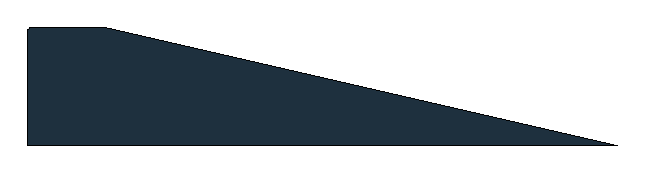
\begin{tikzpicture}
				\draw[fill=HHS_GRAY, line width=0mm, rounded corners=0.25mm] (0,0) -- (\graybandwidth,0) -- (\graybandindented,\graybandheight)-- (0,\graybandheight) -- (0,0);
			\end{tikzpicture}
		}
		\put(500, 775){
\begin{tikzpicture}
				\draw[fill=HHS_GRAY, line width=0mm, rounded corners=0.25mm] (0,0) -- (5,0) -- (7,1.5)-- (-1,1.5) -- (0,0);
			\end{tikzpicture}
		}
		% \put(\hhslogox,\hhslogoy){\includegraphics[scale=0.4]{"graphics/thuas_logo"}}
		%\put(540,781){\includegraphics[scale=0.075]{"./graphics/cam"}}
		\put(250,792){\textcolor{HHS_GRAY}{\Large{\fontfamily{ptm}\sffamily\selectfont \textbf{Project aandachtspunten}}}}
		\put(250,776){\textcolor{HHS_GRAY}{\small{\fontfamily{ptm}\sffamily\selectfont \textbf{Door Mark Schrauwen}}}}
		% \put(345,805){\textcolor{HHS_GRAY}{\Large{\fontfamily{ptm}\sffamily\selectfont Practicumverslag}}}
		% \put(230,780){\textcolor{HHS_GRAY}{\Large{\fontfamily{ptm}\sffamily\selectfont \textbf{ELCA1-T1, Elektronica1, Mechatronica}}}}
		%\put(355,780){\textcolor{HHS_GRAY}{\Large{\fontfamily{ptm}\sffamily\selectfont 16021908 - MeH3}}}
	}
}

\setlength{\headheight}{0pt} % fixes \headheight warning
\fancypagestyle{frontpage}{%
	\newgeometry{top=2cm,bottom=2cm,right=2cm,left=2cm}
	\fancyhead{}
	\renewcommand{\headrulewidth}{0pt}

	%OLD = 346 / 194

	\ClearShipoutPicture
	\AddToShipoutPicture
	{
		\put(349.5,663){
\begin{tikzpicture}
				\fill [HHS_GRAY] (0pt,0pt) rectangle (190.5pt,70pt);
			\end{tikzpicture}}
		\put(56.5,663){
\begin{tikzpicture}
				\fill [HHS_GRAY] (0pt,0pt) rectangle (28.5pt,70pt);
			\end{tikzpicture}}
		\put(95,650){\includegraphics[scale=0.322]{"graphics/qing_logo"}}
		\put(400,40){\includegraphics[scale=0.15]{"graphics/hhs"}}
		\put(50,65){\textcolor{black}{\normalsize{\fontfamily{ptm}\sffamily\selectfont QING Mechatronics BV}}}
		\put(50,50){\textcolor{black}{\normalsize{\fontfamily{ptm}\sffamily\selectfont Westervoortsedijk 73, 6827 AV, Arnhem}}}
	}
}

\setlength{\headheight}{0pt} % fixes \headheight warning
\fancypagestyle{plain}{%
	\newgeometry{top=8cm,bottom=2.5cm,right=4cm,left=4cm}
	\fancyhead{}
	\renewcommand{\headrulewidth}{0pt}
}

\hyphenpenalty 10000
\exhyphenpenalty 10000

\begin{document}
\captionsetup[table]{labelsep=endash}
\captionsetup[figure]{labelsep=endash}

%Title in sans-serif, no page numberbering
\pagenumbering{gobble} % turn of page numbering
\pagestyle{default}


\section{Introduction}
Dit document bevat een aantal aandachtspunten en tips m.b.t. een Mechatronica project.
Gebruik de informatie als 'checklist' aan het begin en einde van een project.


\section{Communicatie}
\begin{itemize}
      \item Zet in het onderwerp van een email altijd een Projectnaam. Bijvoorbeeld: \textit{Project RVD}, \textit{Project Assistive device}
      \item Zet je groepsnaam in het onderwerp. Bijvoorbeeld: \textit{A1} of \textit{C2}
      \item Zet het \underline{specifieke onderwerp} er bij: \textit{toegang tot een lokaal} of \textit{onduidelijkheid m.b.t. de opdracht}
      \item Alles samen zou het onderwerp er zo uit kunnen zien: \newline
            \textbf{\textit{Project RVD, groep A3: vraag over de opdracht}
            }\end{itemize}


\section{Projectuitvoering \& -management}
\begin{itemize}
      \item Lees het projectboek, elke zin! Lees het projectboek in lesweek 3 nog eens!
            %   Lees elke zin! In de 'echte wereld' is er niet zoiets als een \textit{projectboek}.
            %   Daar moet je zelf een project structuren.
            %    Nu krijg je 'een bundel' structuur aangereikt in de vorm van een projectboek.
            %   Je bent 'niet goed wijs' als je daar geen gebruik van maakt.
            % \item Lees het projectboek in lesweek 3 nog een keer helemaal!
      \item Zoek het beoordelingsformulier op.
            Docenten zijn heel erg geneigd een beoordelingsformulier te gebruiken om \textbf{jou} te beoordelen.
            % \item Het beoordelingsformulier geeft focus
      \item Overweeg om gedurende het project in 'wisselende' duo's te werken.
            %   Bijvoorbeeld: Er werkt een duo aan, bijvoorbeeld, de systeem architectuur.
            %   Persoon A van het duo werkt ook weer in een andere duo die aan de lijst met eisen werkt.
            Wat zijn de voordelen van het werken in 'wisselende' duo's?
            Een valkuil in deze werkwijze is: niet goed in de groep afstemmen met elkaar.
            %   In elk duo is 1 persoon 'hoofdverantwoordelijk'. Die persoon is het eerste aanspreekpunt.
            %   De tweede persoon is 'ook verantwoordelijk'.
      \item Het ene leidt tot het andere: \textit{Product Breakdown Structure} (PBS) \textbf{$\rightarrow$} \textit{Work Breakdown Structure} (WBS)
            $\rightarrow$ \textit{Planning}
      \item Een PBS gaat over \textit{dingen} of \textit{deelproducten}. Een WBS gaat over \textit{gedrag} of \textit{activiteiten}
      \item een \textit{agenda} is een hulpmiddel om een vergadering efficient te laten verlopen
\end{itemize}


\section{Samenwerking}
\begin{itemize}
      \item Zorg voor een 'cloud-opslag' en spreek af om altijd 'op de cloud te werken'.
            %   Dat kan ook betekenen dat je lokaal op jouw computer in een folder werkt, die automatisch synchroniseert met 'the cloud'.
      \item Spreek werktijden af. Werken jullie wel/niet in het weekend? Tijdens deze werktijden ben je bereikbaar en beschikbaar!
      \item Maak een projectcontract met afspraken (dit heb je als het goed is al vaker gedaan)
\end{itemize}


\section{Verslaglegging}
\begin{itemize}
      \item Een verslag moet: \textbf{Kort}, \textbf{Duidelijk} en \textbf{Volledig} zijn. Richtlijn aantal pagina's is $30$.
      \item De meest belangrijke verslag onderdelen zijn: de samenvatting, de inleiding en de conclusie. Zorg dat je deze onderdelen 'extreem' goed hebt uitgewerkt
      \item Een samenvatting is het hele 'inhoudelijke' verslag op 1 kantje.
            De \textit{conclusie} en \textit{samenvatting} zijn zelfstandig leesbaar
      \item Zorg voor een \textbf{volledige} titelpagina. Welk project? Welke studenten? Welke groep?, etc.
      \item Bijlagen hoeven niet gelezen te worden. Wat je in de bijlage zet is \textit{zeer waarschijnlijk} bijzaak
      \item Schrijven is schrappen. Het werkt goed om een hoop \textit{bladiebla} op papier te gooien om daarna \textbf{hoofdzaken} te behouden en \textbf{bijzaken} te verwijderen.
      \item Gebruik altijd: hoofdstuk- en paragraafnummering. Zet bij elke tabel/figuur een boven-/onderschrift.
\end{itemize}


\newpage

\begin{figure}[tph]
      \centering
      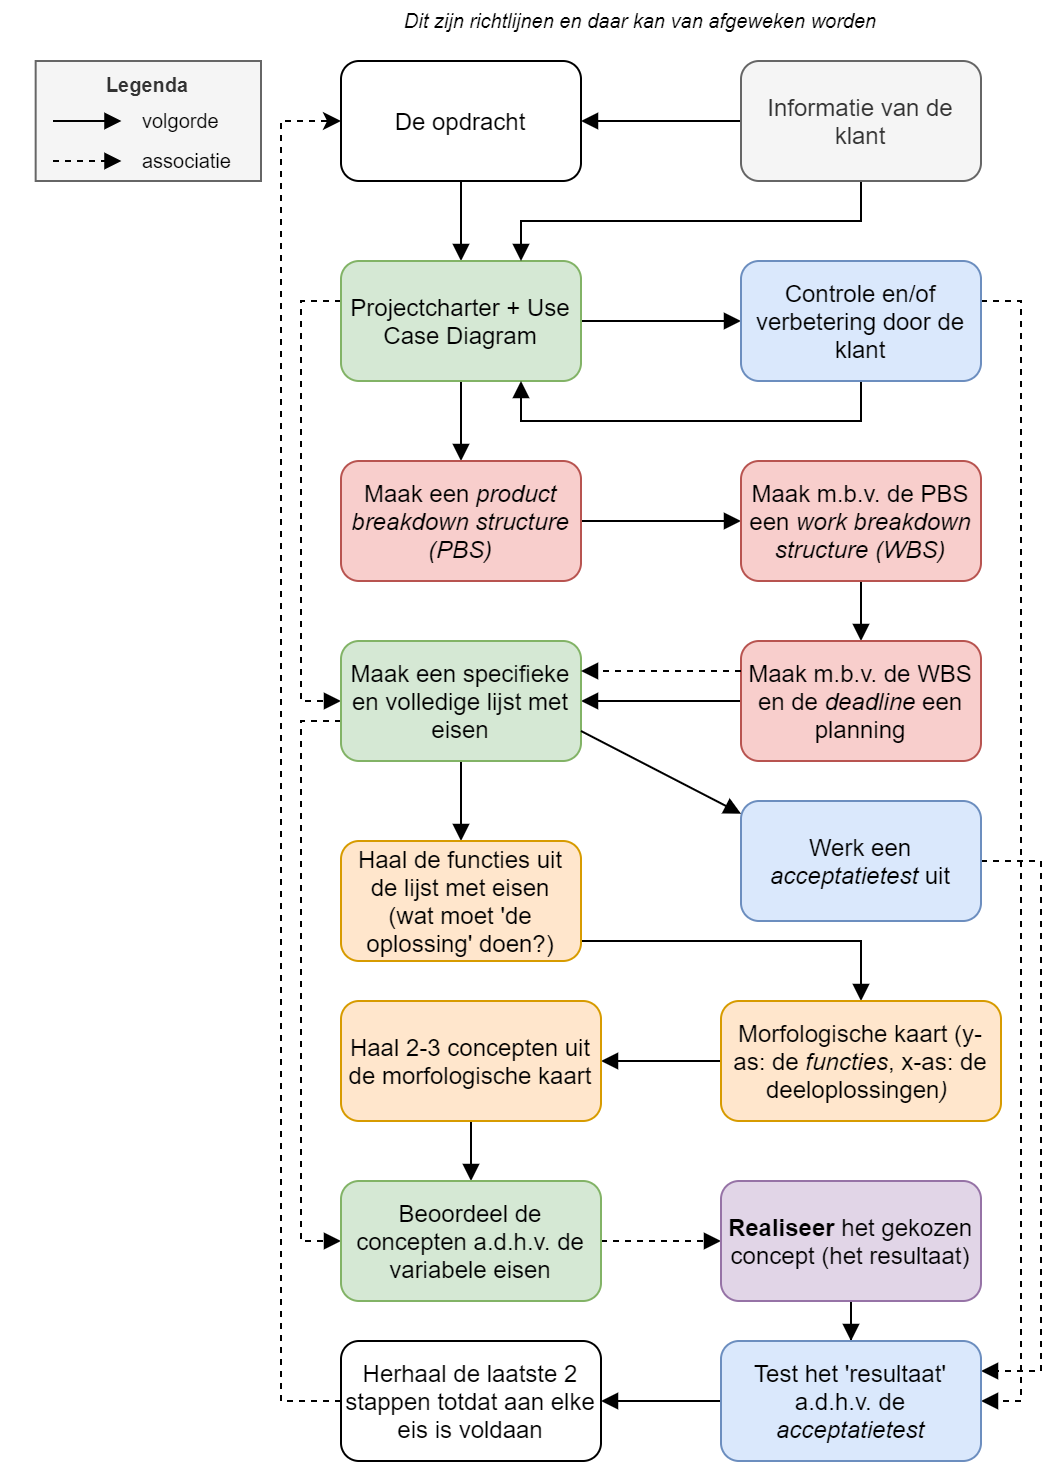
\includegraphics[height=\textheight]{graphics/OntwerpMethodiekMechatronica.png}
\end{figure}


\end{document}